% !TEX root = ../memoria.tex

\chapter{Ensayos y Resultados}

En este capítulo se detallan las pruebas realizadas tanto de manera individual, para comprobar que tanto los componentes de \textit{hardware} como de \textit{software} funcionen como se espera, así como las pruebas de integración realizadas entre los componentes individuales y el \textit{framework} ROS.

\label{Chapter4}

% %----------------------------------------------------------------------------------------
% %	SECTION 1
% %----------------------------------------------------------------------------------------

\section{Pruebas funcionales del hardware}
\label{sec:pruebasHW}

Aquí se describen las pruebas que se realizaron individualmente a cada uno de los componentes del robot.

\subsection{Sensor Microsoft Kinect 360}

% TODO: Capaz mover este parrafito a otro lado

El Kinect es un dispositivo complejo que posee varios componentes internos, todos con diferente identificador USB, que se conectan mediante un cable único. Este cable posee un conector propietario especial que implementa, además de los hilos del estándar USB 2.0, uno de alimentación a 12 VCC y su respectiva tierra.
Por cuestiones de disponibilidad y precio, se procedió a remover manualmente este conector y añadir manualmente un conector estándar USB macho y un plug de alimentación a 12 VCC.

Para testear adecuadamente el funcionamiento del sensor con la adaptación casera, se procedió a conectar el cable USB a un PC con Linux y la alimentación a una fuente externa de 12 VCC. Aquí, se utilizó el comando lsusb, disponible como parte del paquete usb-utils en Ubuntu, y se procedió a listar los dispositivos USB advertidos por el sistema operativo:

% TODO: Agregar captura de pantalla

Una vez corroborado esto, se procedió a verificar que la nube de puntos se esté generando correctamente. Para esto se utilizaron las siguientes herramientas y paquetes de software:

\begin{itemize}

    \item libfreenect: librería de código abierto para el sensor Kinect.
    \item rqt\_image\_viewer: herramienta integrada de ROS para visualizar imágenes RGB y nube de puntos.

\end{itemize}

% TODO: Agregar captura de rqt_image_viewer

\subsection{Unidad de medición inercial InvenSense MPU6050}

Para corroborar el correcto funcionamiento de la IMU se procedió a conectarlo a un Arduino MEGA2560 y se utilizó la librería Adafruit\_MPU6050, la cual se encuentra activamente mantenida por la compañía Adafruit.

Se procedió así, al envío de información RAW via puerto serie y se procedió a graficar, individualmente, cada uno de los componentes de los vectores de aceleración y giro proveídos por el sensor.


%----------------------------------------------------------------------------------------
%	SECTION 2
%----------------------------------------------------------------------------------------

\section{Pruebas funcionales del software}
\label{sec:pruebasSW}

Aquí se describen las pruebas que se realizaron individualmente a cada uno de los módulos de software que componen el sistema.

\subsection{Envío y recepción de datos entre el robot y microcontrolador}

Al tratarse esta de una base móvil comercial, y gracias a la existencia de un documento oficial publicado por el fabricante con información detallada sobre el protocolo de comunicación del robot, se dispone de la gama completa de comandos para manipular los actuadores, así como para leer los sensores disponibles.

Mediante las pruebas descriptas a continuación, se procedió a verificar el subconjunto de periféricos que fueron implementados en el microcontrolador que actúa como interfaz entre el robot y el sistema ROS, corroborando que los mismos funcionen tal y como se describen en el documento mencionado anteriormente.

Para el envío de órdenes desde el microcontrolador hacia el robot, se analizó la respuesta por parte del mismo ante una serie definida de comandos, ante los cuales se corroboró de manera manual que la respuesta sea la esperada.

\begin{table}[h]
    \centering
    \caption{Sub-conjunto de comandos utilizados para testear el correcto funcionamiento del la base móvil}
    \label{comandos hacia robot}
    \begin{tabular}{lll}
        \toprule
        \multicolumn{1}{c}{\textbf{ Comando }} & \multicolumn{1}{c}{\textbf{Descripción}} & \multicolumn{1}{c}{\textbf{Verificación}} \\
        \midrule
        \textbf{START }                        & \begin{tabular}[c]{@{}l@{}}Se inicializa el protocolo\\OpenInterface\end{tabular}                & \begin{tabular}[c]{@{}l@{}}El robot deja de\\ignorar comandos\end{tabular}                 \\
        \textbf{STOP }                         & \begin{tabular}[c]{@{}l@{}}Se finaliza el protocolo\\OpenInterface\end{tabular}                & \begin{tabular}[c]{@{}l@{}}El robot empieza a\\ignorar comandos\end{tabular}                 \\
        \textbf{SAFE }                         & \begin{tabular}[c]{@{}l@{}}El robot pasa a modo\\seguro\end{tabular}                & \begin{tabular}[c]{@{}l@{}}El robot deja de moverse\\si es levantado del suelo\end{tabular}                 \\
        \textbf{FULL }                         & \begin{tabular}[c]{@{}l@{}}El robot pasa a modo\\full\end{tabular}                & \begin{tabular}[c]{@{}l@{}}El robot no deja de\\moverse a menos que\\reciba explícitamente un\\comando STOP\end{tabular}                 \\
        \textbf{DRIVE DIRECT }                 & \begin{tabular}[c]{@{}l@{}}El robot recibe comandos\\de velocidadpara cada\\rueda\end{tabular}               & \begin{tabular}[c]{@{}l@{}}El robot empieza a moverse\\inmediatamente después\\de recibir el comando\end{tabular}                \\
        \textbf{SENSORS }                      & \begin{tabular}[c]{@{}l@{}}Se solicita la lectura del\\estado actualde un sensor \end{tabular}               & \begin{tabular}[c]{@{}l@{}}El robot responde con el\\mensaje correspondiente\\al sensor solicitado\end{tabular}                \\
        \bottomrule
    \end{tabular}
\end{table}

\subsection{Publicación y recepción de mensajes ROS en el microcontrolador}

El proceso en el que se probó la correcta publicación de mensajes desde el microcontrolador hacia ROS, involucró la utilización de las siguientes herramientas integradas del mismo:

\begin{itemize}
    \item rosserial\_python serial\_node
    \item rostopic list
    \item rostopic echo
    \item rostopic hz
    \item RViz
\end{itemize}

Para verificar la existencia de los tópicos anunciados por el microcontrolador fué necesario, primeramente, ejecutar el nodo serial\_node, el cual se encarga de la serialización y des-serialización de los mensajes transmitidos mediante UART o Ethernet, actuando de puente entre el protocolo intermedio de rosserial y ROS.

Luego de haber ejecutado el nodo rosserial en la computadora host, fué posible verificar la existencia de los tópicos invocando el comando `rostopic list`, el cual despliega una lista de los tópicos que se encuentran anunciados.

Una vez conocida la lista de tópicos, es posible reproducirlos en la consola mediante el comando `rostopic echo` así también, es posible verificar su frecuencia de publicación mediante el comando `rostopic hz`.

Luego de verificar la existencia de los mensajes en cada tópico, es posible graficarlos utilizando la herramienta RViz. Esto resulta especialmente útil para mensajes compuestos por varios campos, como los del tipo IMU.

% TODO: Imagen de RViz con una IMU
\begin{figure}[ht]
    \centering
    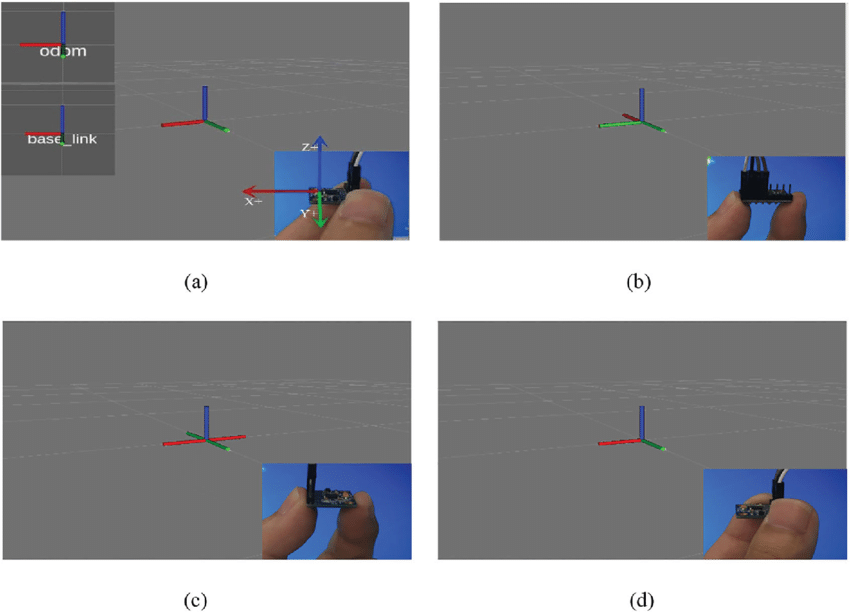
\includegraphics[scale=.4]{./Figures/imu_en_rviz.png}
    \caption{El ángulo \textit{yaw} mostrado en RViz. (a) Posición inicial. (b) Posición rotada a 90 grados. (c) Posición rotada a 180 grados. (d) Posición rotada a 180 grados en sentido anti-horario.}
    \label{fig:cuadradoAzul}
\end{figure}

%----------------------------------------------------------------------------------------
%	SECTION 3
%----------------------------------------------------------------------------------------

\section{Pruebas de integración}

Estas pruebas integran las tareas de alto nivel que se pretende puedan ser utilizadas por los usuarios que adopten la plataforma. Estas involucran la interacción entre todos los componentes del sistema en simultáneo, así como su interacción con el sistema ROS.

Las pruebas se encuentran ordenadas de manera tal que las primeras formen parte de los requisitos para las siguientes y así respectivamente, concluyendo con la prueba de integración

\subsection{Estimador de pose a partir de IMU}

Mediante el nodo imu\_complementary\_filter, integrado como parte del paquete imu\_tools\protect\footnotemark, se procede a procesar la información \textit{raw} proveniente del la IMU. Este nodo provee una estimación de la orientación del robot a partir de lecturas de velocidad angular y aceleraciones, sin la necesidad de un magnetómetro. A su salida, est nodo publica mensajes estándares del tipo sensor\_msgs/Imu\protect\footnotemark, requeridos por el nodo encargado de la localización del robot.

\footnotetext{\url{https://github.com/ccny-ros-pkg/imu_tools}}
\footnotetext{\url{https://docs.ros.org/melodic/api/sensor_msgs/html/msg/Imu.html}}

\subsection{Tele-operación del robot mediante un nodo ROS}

Esta prueba consistió en operar el robot mediante un nodo de ROS, el cual se encarga de publicar mensajes del tipo geometry\_msgs/Twist\protect\footnotemark. Este mensaje es recibido por el robot y aplica los comandos de velocidad a cada una de las ruedas. Para esto se utilizó el nodo teleop\_twist\_keyboard:

\begin{lstlisting}[basicstyle=\ttfamily, keywords={}]
rosrun teleop_twist_keyboard teleop_twist_keyboard.py
\end{lstlisting}

Este nodo permitió comandar el movimiento del robot de forma manual utilizando el teclado de la computadora mediante el uso de los siguientes comandos:

\begin{lstlisting}[basicstyle=\ttfamily, keywords={}]
Reading from the keyboard  and Publishing to Twist!
---------------------------
Moving around:
   u    i    o
   j    k    l
   m    ,    .

q/z : increase/decrease max speeds by 10%
w/x : increase/decrease only linear speed by 10%
e/c : increase/decrease only angular speed by 10%
anything else : stop

CTRL-C to quit
\end{lstlisting}

Esta prueba se consideró satisfactoria el verificar que el robot era efectivamente controlado mediante este nodo. Las velocidades deseadas o \textit{set-points} se verificaron recién durante las pruebas de odometría.

\footnotetext{\url{https://docs.ros.org/melodic/api/geometry_msgs/html/msg/Twist.html}}

\subsection{Odometría}

Esta prueba esta basada en el mismo procedimiento utilizado para tele-operación del robot, con la diferencia que se procedió, además, a comprobar el cálculo de velocidad basado en la lectura arrojada por los encoders. Para esto se utilizó el nodo calculador de odometría elaborado por el autor en lenguaje C++, incluido en el repositorio del presente trabajo.

Para realizar la prueba, se procede de la misma manera que para la de tele-operación, con la diferencia de que se abre, además, el nodo de odometría antes de enviar los comandos de velocidad.

Para lanzar el nodo de odometría utilizamos el siguiente comando:

\begin{lstlisting}[basicstyle=\ttfamily, keywords={}]
rosrun odom_publisher odom_publisher
\end{lstlisting}

Una vez listo, se hace un eco del tópico de odometría, el cual arrojará los valores publicados en la consola. La consigna es comparar los valores de velocidad publicados en el tópico de odometría con los comandos enviados desde el nodo \texttt{teleop\_twist\_keyboard}, debiendo ser éstos similares.

\subsection{Generación de mapa}

Para generar un mapa se utilizó la herramienta gmapping\protect\footnotemark, ofrecida como un paquete de ROS. Esta herramienta es capaz de generar un \textit{occupancy grid} en 2D, muy similar a un plano civil, a partir de las lecturas de \textit{laserscan} generadas por el sensor Kinect, mas la información de odometría colectada por el robot.

\footnotetext{\url{https://wiki.ros.org/gmapping}}

\subsection{Localización en mapa pre-existente}

Esta prueba consistió en colocar el robot en un punto arbitrario del mapa sin proveerle información previa sobre su localización. Aquí el robot debe ser capaz de utilizar sus sensores para reconocer su entorno cercano y reconocer características conocidas entre este y el mapa, siendo capaz de estimar su ubicación. Para este procedimiento se utilizó el mapa generado en el apartado anterior en conjunto con la aplicación RViz para visualizar el estado del procedimiento.

\subsection{Navegación sobre mapa pre-existente}

La navegación sobre un mapa pre-existente esta basada en todas las pruebas de integración anteriores y representa el punto culminante de la serie. Aquí se utilizó la aplicación RViz no solo para visualizar el mapa y la localización del robot, sino también para el envío de puntos de consigna dentro del mapa a los que el robot debe ser capaz de llegar utilizando toda su batería de sensores y estimadores a la vez que evita colisionar con las paredes y objetos presentes.

\label{sec:pruebasIN}